\part{Des projets portés par des institutions culturelles}

 
\chapter{Un contexte universitaire}


Avant tout, il est à noter que les deux stages ont été réalisés de mai à juillet 2020\footnote{Plus précisément du 4 mai au 31 juillet, trois jours par semaine pour le Centre d'Histoire du XIX\up{e} siècle, soit un total de trente-et-un jours et demi de travail, et du 19 mai au 29 juillet, soit un total de vingt jours de travail au Labex OBVIL.}. Suite à la situation sanitaire, nous avons été amenée à réaliser l'intégralité de ces stages en télétravail.

Pour mieux comprendre les objectifs de ces projets, il est important de souligner tout d'abord dans quel cadre ils se sont accomplis. Or, un de leurs points communs est leur contexte universitaire. 


\section{Le Centre de Recherche et d'Histoire du XIX\up{e} siècle}

\subsection{Une institution dédiée à la recherche autour du XIX\up{e} siècle}

Situé dans les locaux de l'université parisienne de la Sorbonne, Paris I, au c\oe ur  du quartier latin, le Centre de Recherche et d'Histoire du XIX\up{e} siècle accueille en son sein les chercheurs qui ont décidé de consacrer leurs travaux au XIX\up{e} siècle. 
Il dispose pour cela d'une bibliothèque de près de huit-mille volumes\footnote{\emph{La bibliothèque}, Site web de l’Université Paris-1 Panthéon Sorbonne, URL :\url{https://www.pantheonsorbonne.fr/unites-de-recherche/crhxix/about-us/thelibrary/}, (visité le 18/06/2020). }.


Fondé par le Professeur Louis Girard (1911-2003), il relève des deux universités de Paris-1 et Sorbonne-Université (anciennement Paris IV)\footnote{\emph{Présentation du Centre}, Site web de l’Université Paris-1 Panthéon Sorbonne, URL : \url{https://www.pantheonsorbonne.fr/unites-de-recherche/crhxix/aboutthecenter/}, (visité le 18/06/2020).}. Il se compose de plus de cent-cinquante personnes, à la fois des professeurs des universités, des maîtres de conférences, divers professeurs agrégés,  allocataires, moniteurs, ATER (Attaché temporaire d’enseignement et de recherche), IATOS (ingénieurs, administratifs, techniciens, ouvriers de service), chercheurs associés et doctorants\footnote{\emph{Présentation du Centre, l’équipe}, Site web de l’Université Paris-1 Panthéon Sorbonne, URL : \url{https://www.pantheonsorbonne.fr/unites-de-recherche/crhxix/about-us/faculty/}, (visité le 18/06/2020).}.
Centre dynamique, il mène de front de nombreux projets.

\subsection{Un Centre dynamique}

Le CRHXIX développe actuellement ses recherches autour de quatre axes principaux\footnote{\emph{Présentation du Centre, les activités de recherche du Centre}, Site web de l’Université Paris-1 Panthéon Sorbonne, URL : \url{https://www.pantheonsorbonne.fr/unites-de-recherche/crhxix/about-us/research-activities/}, (visité le 17/06/2020).}, à savoir en premier lieu, \inquote{Le ``resserrement des sociétés'' : circulations globales et pratiques locales au XIX\up{e} siècle}, en second lieu \inquote{Du moral au social : pratiques et théories de l’enquête. Autour des archives du mouvement leplaysien}, puis sur la problématique \inquote{Citoyennetés, sûretés, sécurités, souverainetés}, et enfin le thème \inquote{Images, imaginaires et écriture de l’histoire}.	

C’est donc dans ce cadre que s’inscrit notre projet scientifique sur \inquote{La correspondance de Frédéric Le Play (1806-1882) : une source pour l’histoire des sciences sociales en Europe}, porté par Sorbonne Université et le CRHXIX.

\subsection{Les acteurs du projet}

L’équipe de recherche de ce projet autour de\inquote{La correspondance de Frédéric Le Play (1806-1882) : une source pour l’histoire des sciences sociales en Europe} est dirigée par Matthieu Brejon de Lavergnée, maître de conférences HDR, et constituée de Philippe Boutry, PR ; Eric Anceau, MCF HDR ; Rémy Hême de Lacotte, MCF ; Marie-Laure Massei-Chamayou, MCF ; Sophie Lhermitte, ingénieur d’études.

De nombreux étudiants, doctorants et stagiaires ont participé de près ou de loin à l’avancement du projet. L’on notera particulièrement la coopération de Madame Margaux Faure, qui a effectué de nombreuses relectures de transcriptions et qui a réalisé elle-même des transcriptions, ainsi que Monsieur Edouard Coquet. Tous deux ont participé aux journées de formation à l’École Nationale des Chartes (ENC) autour de Transkribus, afin de prendre en main les outils qui nous sont nécessaires pour l'avancement de notre projet sur l'édition numérique de la correspondance de Le Play, outils qui seront présentés plus particulièrement dans la troisième partie.

Lors de notre stage, nous avons été surtout amenée à collaborer avec le chef actuel du projet, Monsieur Rémy Hême de Lacotte, avec les avis de Monsieur Matthieu Brejon de Lavergnée à l'origine du projet, et l'ingénieur d'études Madame Sophie Lhermitte\footnote{C'est avec eux que nous avons fait des points réguliers sur l'avancement de notre travail.}. 

\subsection{Partenaires susceptibles d’être mobilisés}

Parmi les partenaires du projet, mobilisés ou susceptibles de l'être, figurent notamment l'Institut universitaire de France (IUF), le Labex EHNE (Écrire une histoire nouvelle de l’Europe), l'École des Chartes (ENC), le Sénat, l'Académie des Sciences morales et politiques, le Centre de sociologie des organisations-Sciences Po et la revue \emph{Les Études Sociales}.

\subsection{Soutiens financiers}
	
Qui dit projet dit financement.
Le projet a reçu un financement du GIS Collex-Persée dans le cadre des appels à projets lancé en 2018 pour soutenir la numérisation de corpus pour la recherche. Il est aussi soutenu par le Labex EHNE. 
Les formations à l’ENC ont été financées par un prêt Collex.

C'est donc dans ce contexte universitaire que s'inscrit notre projet d'édition numérique de la correspondance de Frédéric Le Play. 

Qu'en est-il du contexte du projet ELICOM ?

\section{Le Labex OBVIL}

\subsection{Un laboratoire d'excellence pour les humanités numériques}

Le projet ELICOM (Éditer, Lire des Correspondances Multidisciplinaires) relève, lui aussi, de la Sorbonne. Il est porté par le Labex (laboratoire d'excellence) OBVIL (Observatoire de la vie littéraire), qui est affilié à Sorbonne Université.

Si le CRHXIX est un centre de recherche, le Labex OBVIL est quant à lui un laboratoire de recherche. Même si le terme centre ou laboratoire peut être considéré comme à peu près équivalent, ce dernier a une connotation plus scientifique, et il est par ailleurs classé laboratoire d'excellence. En effet, le Labex OBVIL est très investi dans les humanités numériques. Il regroupe les laboratoires de littérature de l'Université Paris Sorbonne et s'articule avec le Laboratoire Informatique de l'Université Pierre et Marie Curie\footnote{\emph{Laboratoire d'excellence OBVIL}, Site web de l'enseignement supérieur et de la recherche, URL : \url{https://cache.media.enseignementsup-recherche.gouv.fr/file/Fiches_Labex_2/63/8/OBVIL_207638.pdf} (visité le 04/09/2020).}.

Le Labex OBVIL réunit près de quatre cents chercheurs (PR, DR, MCF, CR, Doctorants, post doctorants) répartis dans 24 projets de recherche. Fort d'une équipe de six ingénieurs et d'un soutien administratif à la recherche, délibérément transdisciplinaire, puisqu'il conçoit des outils de numérisation et d'édition, de fouille de texte, d'alignements de texte, de visualisation, le Labex OBVIL mène une recherche novatrice, concevant des humanités numériques littéraires, où littérature et informatique se façonnent mutuellement\footnote{\emph{Observatoire de la vie littéraire}, Site web de l'ANR, URL : \url{https://anr.fr/ProjetIA-11-LABX-0059} (visité le 04/09/2020).}. 

Depuis 2016, il se consacre à des données massives (création de la Très Grande bibliothèque\footnote{\emph{API et jeux de données}, Site web de la BNF, URL : \url{http://api.bnf.fr/mise-disposition-de-la-tres-grande-bibliotheque-du-labex-obvil} (visité le 04/09/2020).}, 130 000 documents), avec le partenariat de la Bibliothèque nationale de France (BNF), et à la conception d'ontologies des corpus critiques et au \emph{text mining}\footnote{\inquote{Le \emph{text mining} est l'ensemble des techniques et méthodes destinées au \emph{traitement automatique} de \emph{données textuelles en langage naturel}, disponibles sous forme informatique, en assez grande quantité, en vue d'en \emph{dégager et structurer le contenu, les thèmes} dans une perspective d'analyse rapide (non littéraire), de découverte d'informations cachées ou de prise automatique de décision. Voir Stéphane Tufféry, \emph{Data mining et statistique décisionnelle}, 4\up{e} édition, Paris, 2012,
p. 2.}}.

\subsection{De nombreux partenaires}

Le Labex Obvil s'entoure pour mener à bien tous ses multiples projets. Il a de nombreux partenaires parmi lesquels on compte le Centre d'étude de la langue et des littératures françaises (CELLF), le Centre de recherche en littérature comparée (CRLC), le Centre de Recherches Interdisciplinaires sur les Mondes Ibériques Contemporains (CRIMIC),  Civilisation et littérature d’Espagne et d’Amérique (CLEA), le Programme de Recherches Interdisciplinaires sur le Théâtre et les Pratiques scéniques (PRITEPS), Voix Anglophones : littérature et esthétique (VALE), l' Equipe Littérature et Culture italiennes\footnote{\emph{Accueil}, Site web de l'Observatoire de la vie littéraire, URL : \url{http://obvil.sorbonne-universite.site/obvil/presentation} (visité le 04/09/2020).}.

C'est donc dans ce contexte particulièrement favorable de recherche scientifique en humanités numériques que s'inscrit un de ses nombreux projets : ELICOM.

\subsection{Les acteurs du projet}

L'équipe travaillant plus spécifiquement sur le projet ELICOM est sous la direction scientifique de Monsieur Glenn Roe - directeur du Labex OBVIL - avec la participation de Monsieur Arthur Provenier, ingénieur d'études, et de Madame Camille Koskas agrégée de lettres modernes en contrat post-doctoral. 

Lors de ce stage, nous avons donc bénéficié de l'encadrement scientifique et technique du Labex OBVIL, et plus spécifiquement de Monsieur Arthur Provenier, qui a également proposé l'aide de ses conseils et avis pour le projet du CRHXIX.\\

C'est donc dans ce contexte universitaire de centre et laboratoire de recherche que se sont développés nos deux projets en humanités numériques. Tous deux sont des projets d'édition numérique de correspondance, sur des corpus du XIX\up{e} siècle. Malgré ces points communs, ils présentent néanmoins des caractéristiques et mises en pratique différentes. Il convient donc de mieux considérer, dans un deuxième chapitre, la nature de ces projets avant de voir leurs sources.




\chapter{Deux projets ambitieux}

\section{L'édition numérique de la correspondance de Frédéric Le Play}

Penchons-nous tout d'abord sur le projet porté par le CRHXIX, à savoir l'édition numérique de la correspondance du sociologue Frédéric Le Play (1806-1882).
Il sera nécessaire avant tout de comprendre quel est cet homme pour mieux saisir pourquoi il est pertinent de publier sa correspondance aujourd'hui.


\subsection{Au service de l'histoire des sciences sociales}
Ce projet d'édition numérique de la correspondance est au service de l'Histoire, et en particulier de l'histoire de la sociologie. L'on voit en ce sens combien, dans les humanités numériques, toutes ces technologies élaborées sont au service de la culture et des humanités. Comme nous l'avons vu plus haut, notre projet s'inscrit dans l'axe de recherche du CRHXIX intitulé \inquote{Du moral au social : pratiques et théories de l’enquête. Autour des archives du mouvement leplaysien} .

\subsubsection{Autour des archives du mouvement leplaysien} 

L’objet d’un axe \inquote{Du moral au social : pratiques et théories de l’enquête. Autour des archives du mouvement leplaysien} est triple : \textbf{rendre accessible} un corpus d’enquête original et encore sous-exploité par une saisie numérique et une édition en ligne ; \textbf{appréhender}, dans les procédures d’enquête, le lien entre société et morales du XIXe siècle : Le Play lui-même relève, on le sait, pour partie du positivisme comtien et pour partie du traditionalisme bonaldien, mais ses disciples et imitateurs obéissent à des logiques diverses au point de former pour certains un courant dissident de la science sociale ; \textbf{analyser} enfin le legs de l’enquête leplaysienne aux sciences sociales en gestation au tournant des XIXe et XXe siècle, sociologie en premier lieu, mais aussi psychologie sociale et histoire des mentalités collectives.

Cet axe, centré sur l’Europe et les États-Unis des années 1850-1920, aurait une dimension éditoriale, historique et historiographique ; il pourrait réunir, autour de l’archive leplaysienne, les contributions de plusieurs disciplines, histoire, sociologie, droit, philosophie, économie, statistique.
Il s’agit donc de donner accès à ces fonds dispersés et parfois peu accessibles en les numérisant et en les mettant en ligne, et de transcrire les lettres pour produire une édition électronique du corpus\footnote{\emph{Axe 2 : Du moral au social : pratiques et théories de l'enquête. Autour des archives du mouvement leplaysien.}, Site web du CRHXIX, URL : \url{https://www.pantheonsorbonne.fr/unites-de-recherche/crhxix/about-us/research-activities/area2/} (visité le 15/06/2020).}.

Pour mieux en saisir toute la portée, il convient d'apprécier qui est Frédéric Le Play.

\subsubsection{Le Play, un sociologue méconnu}

Parmi les personnages qui ont eu leur rôle à jouer dans l'histoire, mais qui sont souvent trop oubliés, figure Frédéric Le Play. À nous de le redécouvrir à travers sa vie, son \oe uvre et son réseau, puisque tout l'objet de notre projet est de les mettre en lumière.\\

Né le 11 avril 1806 dans le Calvados, Frédéric Le Play passe son enfance et ses études entre la Normandie et Paris. À 19 ans, il intègre l'École Polytechnique, où il rencontre les saints-simoniens Michel Chevalier et Jean Reynaud\footnote {Antoine Savoye, « LE PLAY FRÉDÉRIC -
(1806-1882) », \emph{Encyclopædia Universalis}, URL : \url{http://www.universalis-edu.com/encyclopedie/frederic-le-play/ (visité le 12/06/2020).}}. C'est à 1830 que remonte sa \inquote{vocation sociale}. 

Lors de sa carrière dans le corps des Mines, entre 1831 et 1856, il fait de nombreux voyages en Europe : Espagne, Belgique, Sud de la France, Italie, Grande-Bretagne, Scandinavie, Suisse, Autriche-Hongrie, Allemagne, ainsi que Russie, ce sont autant de pays qu'il sillonne et où il va pouvoir enquêter.
En effet, il
\begin{quote}
\inquote{
veut fonder la science sociale. Aussi choisit-il de passer par une longue phase d'accumulation d'observations au cours de laquelle il précise son objet – les familles ouvrières –, définit sa méthode – la monographie – et élabore ses techniques : l'établissement du budget familial d'une part, la collecte d'informations auprès des autorités sociales de l'autre. Multipliant, en outre, les voyages, il élargit et systématise son étude comparative\footnote{\emph{Idem.}}}.
\end{quote}
Par ailleurs, ces
\inquote{voyages sont justifiés par son cours à l’École qu’il actualise et la préparation de son ouvrage de science sociale \emph{Les ouvriers européens}, notamment pour la réalisation de monographies\footnote{\inquote{La monographie selon Le Play est donc la matrice de diverses techniques qui sont aujourd'hui employées en sociologie, en ethnographie, en psychologie sociale, en histoire, en géographie humaine, etc.} \emph{Ibid.}} de familles ouvrières}\footnote{\cite{savoye_lp_qqdates}} qu'il considère comme révélatrices de l'\inquote{état social}. À la suite de ces voyages, il publie souvent des mémoires scientifiques où l'on peut suivre l'élaboration de sa pensée.

Cette pensée, il la développe dans nombre de ses ouvrages : avec la \emph{Réforme sociale en France} en 1864, \inquote{Le Play propose une analyse globale de la société française [...] depuis l’organisation de la vie privée jusqu’aux mécanismes administratifs et de gouvernement} proposant des réformes \inquote{étayées sur ses enquêtes et celles effectuées par ses collaborateurs\footnote{\cite{savoye_lp_qqdates}}}. Dans \emph{Les Ouvriers européens}, réédité à la fin des années 1870, Le Play, d'après ses observations, souligne les éléments qui garantissent la stabilité d'une société, qui passe par deux fondements invariables, \inquote{le respect du Décalogue et le règne de l'autorité paternelle}\footnote {Antoine Savoye, « LE PLAY FRÉDÉRIC - (1806-1882) », \emph{Encyclopædia Universalis}, URL : \url{http://www.universalis-edu.com/encyclopedie/frederic-le-play/}}.

De 1857 à 1870, il tient un rôle politique de conseiller d'État, sénateur et réformateur social. Il \oe uvre notamment à la réforme du droit successoral et trouve un appui auprès des catholiques libéraux. Les expositions universelles sont aussi pour lui l'occasion de faire valoir ses idées\footnote{En 1855, il est nommé commissaire général à l'occasion de l'exposition universelle de Paris. \emph{Idem.}}. Par ailleurs, la création des unions de la paix sociale (UPS), sorte de groupements savants et militants, lui permet de faire connaître sa pensée et élargir son influence.

Sa correspondance est aussi un moyen pour lui de faire part à  ses amis polytechniciens du fruit de ses recherches pour en arriver à la Réforme sociale. Il passe de nombreuses heures par jour à s'épuiser dans une correspondance abondante afin de faire germer sa pensée dans les esprits des savants de sa connaissance. 

Par la création de \emph{La Réforme sociale}, en 1881, il se donne une revue pour développer sa pensée et la perpétuer après sa mort qui survient l'année suivante.

Les moyens de diffusion de sa pensée sont donc nombreux, et l'un d'eux, sa correspondance, est donc l'objet de notre projet.


\subsection{Redécouvrir l’un des fondateurs de la sociologie}
\subsubsection{Explorer la méthode scientifique de Le Play, éclairer les conditions d’élaboration des enquêtes}
Comme nous l'avons dit plus haut, Le Play est un précurseur des méthodes d'enquêtes sociologiques de terrain. 
\begin{quote}
    \inquote{Ses principes d'observation
directe de la réalité et de recherche comparative, sa méthode monographique, ses techniques de
quantification par le budget qu'il a appliqués à l'étude systématique des familles ouvrières font
pourtant de lui le premier théoricien de la sociologie de terrain. De plus, sa double activité de haut
fonctionnaire et de sociologue éclaire l'histoire de la sociologie\footnote{\emph{Ibidem.}}}.
\end{quote}

Notre projet scientifique consiste donc à éclairer les conditions d’élaboration des enquêtes qui se multiplient en Europe à partir des années 1840 (Buret, Villermé, Blanqui, Engels…) et qui s’interrogent sur les mutations du monde du travail et la naissance d’un paupérisme de masse, ce que l’on appelait alors la « question sociale ». Or ces enquêtes publiées gomment toute la phase préparatoire, pourtant riche d’enjeux aussi bien épistémologiques qu’idéologiques. Les correspondances représentent une source inexploitée pour étudier cet aspect. En travaillant sur les pratiques savantes d’un groupe d’enquêteurs réunis au sein d’une école « sociologique » relativement homogène, nous pensons pouvoir contribuer de manière pluridisciplinaire à l’histoire des sciences sociales. L’« école » leplaysienne jouit d’un regain d’intérêt historiographique mais sa mémoire demeure relativement effacée par l’école durkheimienne concurrente. Notre projet de recherche promet donc des résultats scientifiques neufs.

\subsubsection{Frédéric Le Play, au croisement de nombreux champs intellectuels}

\begin{figure}[ht]
    \centering
    \caption{Carte mentale de Le Play, \emph{Encyclopædia Universalis}}
    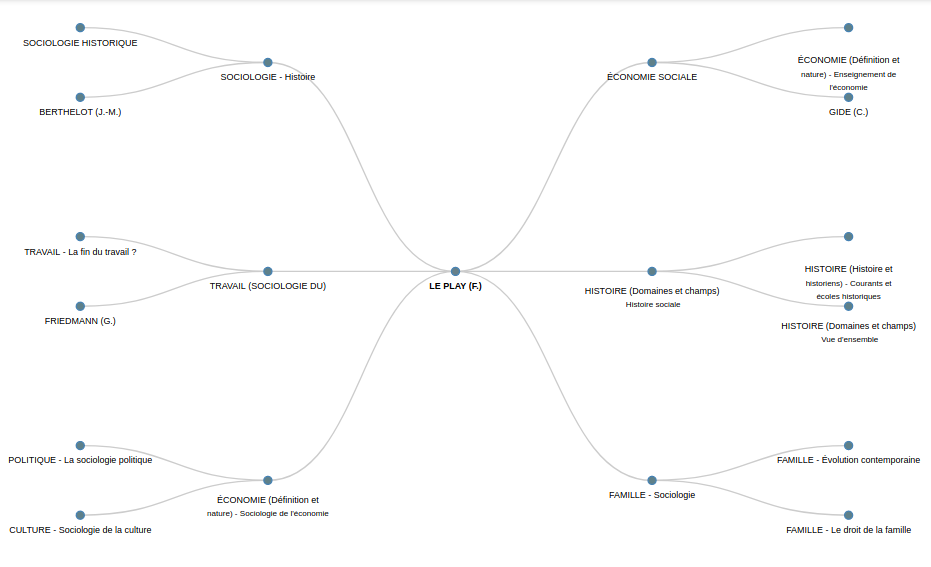
\includegraphics[width=16cm]{carte_mentaleLP}
    \label{carte_mentaleLP}
\end{figure}
Par ailleurs, Frédéric Le Play se trouve au croisement de nombreux champs intellectuels, à nous de voir comment nous pourrons le faire valoir dans notre projet. Il s'agit pour nous de relever un défi pour faire connaître un sociologue méconnu.



Lors de la présentation des sources dans le troisième chapitre, nous détaillerons l'importance des sources qui sont en notre possession ou en cours d'acquisition. 
Avant cela, il importe de présenter le deuxième projet sur lequel nous avons travaillé, au sein du Labex OBVIL.




\section{ELICOM}

A travers ELICOM, le Labex OBVIL 
\begin{quote}
\inquote {propose une recherche inédite sur la question de la valeur littéraire, envisagée au travers de l'étude de grands corpus numérisés qui prennent en compte, non seulement les textes eux-mêmes mais les circonstances et les modalités de leur publication et de leur réception\footnote{Laboratoire d'excellence OBVIL, \emph{Site web de l'enseignement supérieur et de la recherche}, URL : \url{https://cache.media.enseignementsup-recherche.gouv.fr/file/Fiches_Labex_2/63/8/OBVIL_207638.pdf} (visité le 04/09/2020).}}.
\end{quote}

Si les sources en elles-mêmes nous seront exposées plus en détail dans le chapitre suivant, présentons dès à présent les grands axes du projet\footnote{Cette présentation du projet est largement inspirée des documents qui ont été présentés afin d'obtenir les financements.}.

Retenu par l'appel à projet Émergence\footnote{Voir : Appel à projets Emergence , \emph{Site web de Sorbonne Universités}, \url{https://candidature.sorbonne-universites.fr/index.php?option=com_emundus&view=programme&id=111&Itemid=1521&lang=fr} (visité le 07/09/2020)} qui entend consolider l'excellence au c\oe ur des disciplines, accompagner les évolutions interdisciplinaires et ouvrir l'université sur la société, le projet ELICOM se révèle 
être ambitieux et innovant, car il est plus qu'une simple édition numérique de correspondance. 

\subsection{Pour une recherche collective et multidisciplinaire}

Tout d'abord, le présent projet semble s’inscrire dans un mouvement de recherche collective, national ou international. Mais cette inscription en fait bien apparaître la singularité : elle sort du cadre strictement littéraire pour s’ouvrir à des corpus de philosophie, de biologie, de mathématiques. Cette multidisciplinarité répond à la volonté de s’appuyer sur les collaborations institutionnelles, à l’intérieur de Sorbonne Université avec sa Bibliothèque riche en archives scientifiques, avec la Bibliothèque Nationale de France (BNF) dont Gallica offre d’immenses ressources de correspondances éditées en format image, voire en mode texte. Le labex OBVIL poursuit ainsi sa politique patrimoniale de recherche tout en accentuant sa réflexion sur les services qu’il peut offrir à la communauté dans laquelle il s’insère et à la communauté des chercheurs. 

\subsection{Un outil de réflexion et de recherche}

Cela signifie aussi que le caractère innovant du programme ne réside pas dans les correspondances elles-mêmes, même si le labex OBVIL apportera son savoir-faire et son expertise aux spécialistes d’un auteur qui éditent ou souhaitent éditer, au format numérique, une correspondance. Il réside avant tout dans la volonté forte de constituer autour d’un objet théorique – qu’est-ce que correspondre par lettres ?- une communauté de spécialistes venus de disciplines différentes pour penser les besoins éditoriaux en fonction des possibilités offertes par le numérique. La création d’une plateforme d’édition et de lecture répondra aux besoins multidisciplinaires tout en devenant un outil de réflexion et de recherche pour les communautés de chercheur.

L’ambition ultime sera de tester les résultats du présent programme sur des correspondances émanant non plus d’une élite savante, mais de communautés plus ordinaires, familiales, ou socio-professionnelles. Le projet ambitionne ce retour vers la vie ordinaire, sociale, professionnelle, citoyenne. 

\subsection{Trois modules}


Ces corpus, une fois édités - ce qui n’est qu’un préalable au projet pris en charge par le Labex OBVIL - forment un premier échantillon multidisciplinaire qui est exploité par les trois modules de la plateforme ELICOM : l’enrichissement, la fouille et l’exploitation.

\subsubsection{Enrichissement}

Ce premier module offre à chaque utilisateur la possibilité d’enrichir les textes édités à l’aide de balises TEI\footnote{Nous reviendrons sur tous ces termes dans la suite du mémoire.}, choisies à partir de ses propres questionnements, et en s’appuyant sur le manuel d’encodage pour correspondances mis au point par le consortium CAHIER\footnote{ Richard Walter (dir.), \emph{L’édition numérique de correspondances – guide méthodologique}, URL :  \url{https://cahier.hypotheses.org/guide-correspondance} (visité le 17/06/2020).}. Il lui permet également d’annoter chaque lettre en collaborant à la mise en place d’un apparat critique comme des notes savantes et des références bibliographiques, et de compléter les métadonnées.
Cet enrichissement participatif permet à terme d’adapter les corpus aux perspectives de recherche de chacun, et de mettre un ensemble de données et de métadonnées à disposition de la communauté scientifique.

\subsubsection{Fouille}

Ce second module ouvre ensuite à la fouille des textes et de leurs métadonnées, par un ensemble d’outils de \emph{text mining}. Il prévoit également un travail de modélisation sémantique, réalisé au cours du séminaire qui accompagne le développement de la plateforme, et qui s’appuie à la fois sur une construction systématique de ressources linguistiques à caractère polémique et sur des corpus de correspondances annotés manuellement par des experts. L’enjeu est de pouvoir exploiter ces données par des outils du Traitement automatique des langues (TAL) dans le but d’effectuer :
\begin{itemize}
    \item une analyse sémantique des controverses (identifier les postures et les positionnements de débats, de polémiques, etc.) 
    \item une analyse des enchaînements temporels (différenciant récit de vie et discours)
    \item une analyse thématique (autour des événements publics et privés)
    \item une analyse des rituels de la correspondance (formules de politesse, styles selon le destinataire) 
    \item un repérage des entités nommées\footnote{\inquote{On appelle entité nommée toute expression linguistique qui réfère à une entité unique du modèle de manière autonome dans le corpus.} Voir : Maud Ehrmann, \emph{Les Entitées Nommées, de la linguistique au TAL : Statut théorique et méthodes
de désambiguïsation}, Thèse de doctorat, Université Paris Diderot, 2008, URL : \url{https://hal.archives-ouvertes.fr/tel-01639190} (visité le 07/09/2020).}, etc.
\end{itemize}

L’ensemble de ces fonctionnalités doit permettre une exploration transversale des correspondances par le biais de requêtes croisées (par nature de la lettre, par thématique, par lieu, par âge ou sexe des correspondants, etc.), de manière à conduire l’utilisateur vers certains événements propres à la correspondance épistolaire.

\subsubsection{Exploitation}

Ce troisième module propose différents types de visualisation permettant une représentation et une analyse des données et des métadonnées des correspondances : des nuages de collocations, des réseaux (entités nommées et métadonnées), des cartographies par géolocalisation, des visualisations de relevés statistiques et des visualisations croisées par période et par fréquence de correspondances, par lieu et par auteur, etc.\\

Le projet étant très vaste, nous en sommes encore à la phase d'encodage en XML-TEI. C'est donc cette partie qui nous a été confiée lors de notre stage. Gérer un corpus aussi large est un véritable défi, notamment dans le choix des balises. C'est ce défi que nous avons dû relever. Mais avant cela, il faut penser l'édition. Ce sera l'objet de notre seconde partie. En attendant, il sera bon de considérer quelles sont les sources exploitées pour avoir meilleure vue d'ensemble du projet.




\chapter{Les sources des projets : des correspondances du XIX\up{e} siècle aux formes variées}

Les deux projets auxquels nous avons participé n'ont pas les mêmes caractéristiques tout en ayant de nombreux points communs, comme nous l'avons déjà souligné.

Pour le CRHXIX, l'objectif est de mettre à disposition une correspondance riche mais oubliée et peu connue et reconnue.
Pour OBVIL au contraire, l'objectif est de (re)mettre en valeur une correspondance qui a déjà été publiée, à laquelle on s’est déjà intéressée, qui est déjà en ligne, mais dont on voudrait faciliter l’exploitation, le croisement des sources, l'interopérabilité. 

Pour le projet d'édition numérique de la correspondance de Frédéric Le Play, nous travaillons sur un homme autour duquel se greffe tout un réseau. Pour ELICOM, c'est un réseau en soi que nous mettons en valeur.

Par ailleurs, pour le projet Le Play, c'est une approche plutôt classique d'édition. Pour ELICOM, c'est une démarche innovante.

Enfin, et c'est ce qui fait toute la différence des moyens employés, pour le projet Le Play, nous avons affaire à des manuscrits originaux numérisés ou à numériser, alors que pour ELICOM, nous travaillons sur des éditions imprimées qui ont été numérisées et sont disponibles sur Gallica.

Il est donc temps de présenter ces différents corpus du XIX\up{e} siècle.

\section{La mise en valeur de manuscrits}

Tout d'abord, le CRHXIX est en pleine phase d'acquisition de manuscrits de Frédéric Le Play sous une forme numérisée. .

La correspondance de Le Play est relativement dispersée. Elle se trouve principalement en Europe, plus particulièrement en France, mais certains manuscrits sont conservés en Suisse et en Italie par exemple. 

Il s'agit donc de contacter les différents lieux de conservation de ces manuscrits - bibliothèques,  archives privées et publiques etc. - demander leur numérisation en vue de leur transcription et encodage pour la future mise en ligne du manuscrit et de sa transcription.

Ce travail a été déjà bien entamé. 
Un premier inventaire provisoire, de plus de deux-mille lettres, a déjà été réalisé en 2005 par Stéphane Baciocchi et Antoine Savoye - spécialiste reconnu de Frédéric Le Play - paru dans la revue des \emph{Études sociales}\footnote{\cite{inventaire}}. Nous nous y sommes référée dans notre travail de prise en main du projet pour avoir une vue d'ensemble des sources. Nous nous y reportons donc également pour cette présentation des sources. 

\subsection{Trois fonds familiaux principaux}

Les archives de Frédéric Le Play ont été localisées dans trois fonds principaux : au château de Ligoure (Haute-Vienne), à la Bibliothèque de l'Institut de France (BIF) à Paris, ainsi qu'à la Société d'économie et de science sociales (SESS) à Paris.

\subsubsection{Château de Ligoure (Haute-Vienne)}
En 1856, Frédéric Le Play achète le domaine de Ligoure, y établissant une famille-souche\footnote{Principe selon lequel \inquote{l'un des fils demeure avec sa femme et ses enfants dans le foyer paternel en attendant la succession}, développé par Frédéric Le Play, expliqué ici par Emmanuel Todd, \inquote{Les familles dans l'Histoire}, \emph{Herodote.net}, URL : \url{https://www.herodote.net/Les_familles_dans_l_Histoire-article-1287.php} (visité le 08/09/2020).} à travers son fils, Albert Le Play. Frédéric Le Play y séjourne pendant l'été et retourne dans sa résidence parisienne durant l'hiver.

D'après l'inventaire réalisé par Antoine Savoye et Stéphane Baciocchi, on constate que
\begin{quote}
\inquote{de nombreuses lettres de Frédéric à son fils (1865-1881), notamment celles dans lesquelles il est question de la gestion du domaine agricole, y sont encore aujourd'hui conservées et propriété de l'arrière petite-fille d'Albert, Madame Thomas-Mouzon. Elles voisinent, dans les tiroirs et placards de la bibliothèque, avec celles que F. Le Play adressa à sa belle-fille, son « héritière-associée » (1867-1880), et quelques autres lettres des années 1866-1876. En attendant un inventaire plus précis de ce fonds, on peut d'ores et déjà penser que toutes les correspondances restées à Ligoure sont une partie de celles qui y ont été adressées après 1864\footnote{\cite{inventaire}}.}
\end{quote}

\subsubsection{Bibliothèque de l'Institut de France (Paris)}

Le fonds conservé à la BIF lui a été confié par Jean Albert Le Play, arrière petit-fils de Frédéric Le Play, en 1946. Il comporte un millier de lettres datées des années 1832-1882 et des liasses de notes manuscrites et de papiers divers.

Certaines sont adressées à Victor Legrand, directeur général des ponts et chaussées et des mines, au cours ou au retour de ses missions à travers l'Europe (1836-1846).
Il constitue le seul fonds public qu'il nous reste de Le Play et laisse à entendre que un bon nombre de papiers ont disparu. Le gros de la correspondance conservée est en lien, d'une part, avec les éditions successives et la diffusion de ses ouvrages la \emph{Réforme sociale en France}, l'\emph{Organisation du travail}, l'\emph{Organisation de la famille} et, d'autre part, avec la mise en place des UPS. Cet ensemble est daté des années 1860 et 1870. 

Comme le soulignent Antoine Savoye et Stéphane Baciocchi, 
\begin{quote}
    \inquote{le fonds public, ouvert depuis 1946 aux chercheurs, est celui où ont puisé tous les travaux de première main sur Le Play, sans toujours s'interroger explicitement sur les effets de sources, en l'espèce particulièrement discontinues et composites. On pourrait ici pointer l'inadéquation des récits biographiques linéaires fondés sur un tel matériau\footnote{\cite{inventaire}}.}
\end{quote}
D'où l'intérêt de notre travail qui permettra de mettre en ligne non seulement ce fonds déjà ouvert, mais aussi nombre de lettres encore inconnues du grand public et qui permettront de faire des recherches plus cohérentes sur Le Play et donneront l'occasion de voir apparaître de nouvelles études plus complètes.

\subsubsection{Société d'économie et de science sociales (Paris)}

Jean Albert Le Play conservait encore certaines lettres de son ascendant. Celles-ci ont été confiées en 1986 à la SESS. On y trouve plus de 200 lettres que Frédéric Le Play adressa à sa mère Rosalie Le Play-Auxilion (1833) et à sa femme Augustine Le Play-Fouache (1837-1877).\\

Ces trois fonds familiaux constituent 1167 lettres adressées à 49 correspondants.

\subsection{Des fonds dispersés à travers l'Europe}

A côté de ces trois massifs, la correspondance est particulièrement éclatée dans de nombreuses bibliothèques et centres d’archives, tant en France (Archives nationales, Bibliothèque nationale de France, bibliothèque Thiers, etc.) qu’à l’étranger (Angleterre, Belgique, Italie, Russie, etc.).

Les fonds complémentaires sont les ouvrages de Le Play, les enquêtes publiées, les revues du mouvement. Une large partie est disponible sur Gallica (\emph{La Réforme sociale en France}, 1864 ; \emph{Les Ouvriers européens}, 6 volumes entre 1877 et 1879 ; revue \emph{La Réforme sociale}, 1881-1934, etc.)\\
   
Enfin, on constate malheureusement que la correspondance autour de Le Play est lacunaire. Ainsi, aucune correspondance avec Albert de Saint-Léger et Adolphe Focillon, pourtant acteurs essentiels des premiers développement de la science sociale, n'a été retrouvée. Nous n'avons pas non plus trouvé trace d'Alexis Delaire, alors qu'il a eu un grand rôle à jouer dans l'organisation des UPS.

Par ailleurs, les correspondants étrangers sont rares, et aucune correspondance russe n'a été retrouvée, on pense surtout à Anatole de Demidoff, \inquote{commanditaire et employeur de Le Play durant une vingtaine d'années et qui lui a ouvert les portes de la Russie, découverte essentielle\footnote{\cite{inventaire}}.}


\subsection{Une correspondance au service de l'Histoire}

Le corpus, bien qu'incomplet, est largement prometteur. On y discerne déjà des thèmes principaux\footnote{Ces thèmes ont été relevés toujours par l'inventaire déjà nommé de 2006 que nous paraphrasons.}, qu'il est important d'avoir en mémoire pour les futurs choix éditoriaux :

\begin{itemize}
    \item La genèse des Ouvriers européens éclairée par la correspondance avec Jean-Baptiste Dumas et Augustin Cochin.
    \item L'organisation interne de la Société d'économie sociale (sur laquelle on ne possède pas d'archives pour le XIX\up{e} siècle) révélée par la correspondance avec Louis de Kergorlay.
    \item La volonté d'intervention publique de Le Play qui se manifeste à travers ses relations avec les catholiques libéraux (correspondance avec A. Cochin, Mgr Dupanloup et particulièrement Charles de Ribbe.
    \item La fondation expérimentale d'une « famille-souche » telle qu'elle apparaît dans la correspondance avec son fils, Albert.
    \item La conception du rôle de l'Église et la place de la religion dans la société (correspondance avec le père Hyacinthe). On y voit les importantes questions qu'y se posent autour du Concile Vatican I.
    \item La praxis réformatrice dont, lettres après lettres, Le Play précise sa conception à des interlocuteurs comme Emmanuel de Curzon et l'Écossais, David Urquhart.
\end{itemize}

Nous pouvons conclure, toujours avec Messieurs Antoine Savoye et Stéphane Baciocchi, que nous avons là \inquote{de quoi alimenter un vaste programme de travail, tant sur l'émergence des sciences sociales que sur les évolutions de la pensée sociale dans la France du Second Empire et de la III\up{e} République commençante\footnote{\cite{inventaire}}.}

\subsection{Nature des sources et première prise en main du projet}

L'ensemble de cette correspondance compte 2091 lettres échangées entre Frédéric Le Play et 94 correspondants entre 1837 et 1882.
Il s'agit donc de ne pas se perdre dans cette correspondance hétéroclite, à la fois active et passive.

Les premiers jours du stage ont donc été consacrés à un recensement des lettres qui nous ont été confiées\footnote{Le stage étant en télétravail, nous avons dû procéder à un versement par WeTransfer, service de transfert de fichiers en ligne.}.\begin{figure}[ht]
    \centering
    \caption{Fonds numérisés, extrait de l'inventaire}
    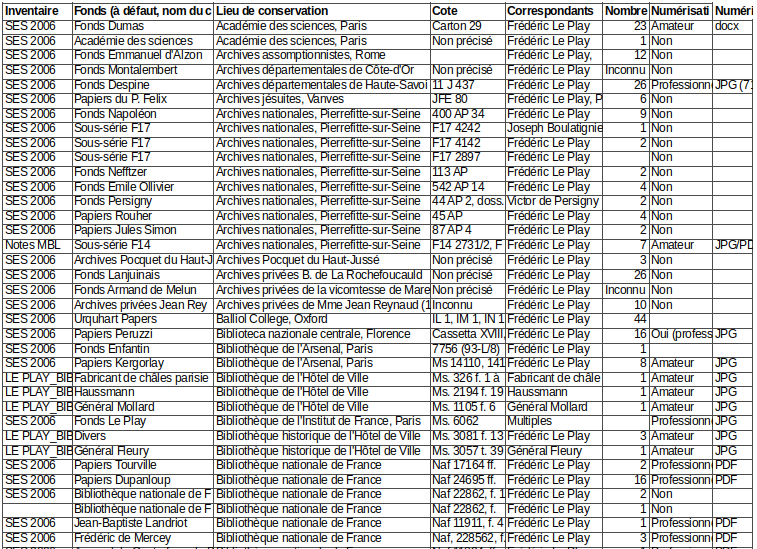
\includegraphics[width=16cm]{images/inventaire_numerisationsRHDL.png}
    \label{inventaire_numerisationsRHDL}
\end{figure} En effet, le seul document de référence pour comprendre les archives était l'inventaire de 2005. Nous ne disposons pas d’inventaire ou de description précise des fonds que nous avons pu récolter. Nous avons donc établi un tableau excel pour discerner quelles correspondances nous devions traiter en priorité, selon la qualité des numérisations que nous avions en notre possession. 
Nous nous sommes concentrée particulièrement sur les manuscrits écrits de la main de Frédéric Le Play afin de pouvoir commencer notre travail sur Transkribus, point que nous développerons davantage dans la deuxième partie.

Le CRHXIX est encore dans une phase d'acquisition des sources. Il en possède déjà des photocopies, matériau peu rentable pour notre future mise en ligne. Il détient également des numérisations, qui sont dans l'ensemble de qualité. Enfin, il possède des photos de médiocre qualité. Il sera nécessaire d'en demander par la suite les numérisations aux institutions en question.

Par la suite, nous avons eu accès à un fichier récapitulatif des transcriptions qui nous a été fort utile, et au cours de notre stage, un membre de l'équipe a également réalisé un fichier excel dont l'objectif était de faire un point sur la qualité des numérisations. Nous en trouvons ici\footnote{Fig. 3.1} un aperçu qui nous permet de voir l'ampleur des fonds.

La prise en main du projet est donc déterminée par la nature des sources en notre possession. Ceci vaut aussi bien pour le CRHXIX que pour le Labex OBVIL.





\section{De l'édition papier à l'édition numérique}

Pour ELICOM, les sources du projet sont bien différentes. En effet, bien que ce soient également des lettres du XIX{e} siècle, nous travaillons cette fois-ci non plus sur la source directement ou sur sa numérisation, mais sur des imprimés qui ont été numérisées. Pour cela, Gallica est une mine inépuisable ou presque.

\subsection{Gallica, une mine de savoirs}

Gallica est la bibliothèque numérique de la BNF. Elle regroupe plus de six millions de documents, livres au format Epub, journaux, revues, images, enregistrements sonores, cartes, manuscrits et vidéos. 

Parmi ces multiples documents, on trouve de nombreux ouvrages numérisés, dont d'anciennes éditions de correspondances du XIX\up{e} siècle. Ce sont elles qui ont été choisies dans le cadre du projet ELICOM pour être traitées afin d'être plus accessibles aux chercheurs et plus aisément fouillées. 

Pour notre projet, un cahier des charges avait déjà était dressé il y a deux ans, mettant en exergue les sources intéressantes repérées sur le catalogue de la BNF, et redirigeant vers les sources présentes sur Gallica. Plusieurs noms ressortent de cette analyse.

\subsubsection{Pierre-Joseph Proudhon}

Proudhon (1809-1865) reflète à lui seul la volonté de multi-disciplinarité d'ELICOM. Polémiste, journaliste, économiste, philosophe, politique et sociologue français, sa correspondance est riche de quatorze volumes\footnote{ \emph{Correspondance de P.-J. Proudhon}, \emph{BNF Catalogue général}, URL : \url{https://catalogue.bnf.fr/ark:/12148/cb35438908j} (visité le 08/09/2020).}. Précurseur de l'anarchisme, il est le seul théoricien révolutionnaire du XIX\up{e} siècle à être issu du milieu ouvrier.\\

Durant notre stage, nous avons pu réaliser l'extraction du premier volume, soit près de cent lettres. Les correspondants sont relativement nombreux. On y trouve notamment le journaliste et premier disciple de Fourier, Just Muiron (1787-1881),  le philologue Paul Ackermann (1812-1846) et l'orientaliste, sinologue et poète Guillaume Pauthier (1801-1873). Nous y reviendrons plus en détail dans la troisième partie de ce mémoire.

\subsubsection{Louis Pasteur}

Avec Louis Pasteur (1822-1895), dont nous avons retenu quatre volumes de correspondance\footnote{ \emph{Correspondance de Pasteur, 1840-1895}, \emph{BNF Catalogue général}, URL : \url{https://catalogue.bnf.fr/ark:/12148/cb32510650x} (visité le 08/09/2020).}, nous sommes face à un corpus plus scientifique, qui souligne encore une fois la volonté trans-disciplinaire d'ELICOM.

Néanmoins, nous devons préciser que nous n'avons pas eu à traiter ce correspondant durant notre stage.

\subsubsection{George Sand}

Nous n'avons pas non plus traité la correspondance de George Sand (1804-1876), riche de six volumes\footnote{\emph{Correspondance : 1812-1876 / George Sand, BNF Catalogue général}, URL :\url{https://catalogue.bnf.fr/ark:/12148/cb31293789z} (visité le 19/05/2020).}, correspondance cette fois d'une femme de lettres, depuis ses huit ans jusqu'à sa mort à l'âge de soixante-douze ans.

\subsubsection{Alphonse de Lamartine}

La correspondance de Lamartine (1790-1869), qui comporte six volumes\footnote{ \emph{ Correspondance de Lamartine, BNF Catalogue général}, URL : \url{https://catalogue.bnf.fr/ark:/12148/cb30725428p} (visité le 19/05/2020).}, est celle sur laquelle nous nous sommes le plus attardée, puisque c'est par elle que nous avons commencé notre stage et que nous nous sommes familiarisée avec les procédures à suivre.

Nous nous sommes attelée à l'extraction du premier volume, comportant près de cent lettres, où Lamartine correspond avec ses meilleurs amis, Prosper Guichard de Bienassis et Aymon de Virieu.
Le deuxième volume comporte un nombre plus important de correspondants, parmi lesquels figurent encore Aymon de Virieu, et aussi Laurent de Jussieu, Fortuné de Vaugelas, Éléonore de Canonge, la marquise de Raigecourt, le baron de Vignet, le comte de Saint-Mauris, le duc de Rohan, l'abbé Dumont et Eugène de Genoude.    

\subsubsection{Félicité de Lamennais}

L'Abbé Félicité de Lamennais (1782-1854) présente une correspondance active forte de deux volumes\footnote{\emph{ Correspondance de Lamennais, BNF Catalogue général}, URL : \url{https://catalogue.bnf.fr/ark:/12148/cb30728369q} (visité le 08/09/2020).}, adressée pour ce qui est du premier volume que nous avons traité, pour la plupart à des personnes de son rang, telles que Mademoiselle Cornulier de Lucinière, Monsieur le Comte de Senfft et Madame la Comtesse de Senfft, ou encore au Marquis de Coriolis\footnote{Les correspondants sont nommés avec leurs titres dans cette correspondance.}. Un volume représente en réalité trois tomes, et donc près de deux-cent lettres d'une longueur assez importante en général. Le premier volume regroupe la correspondance de 1818 à 1823. Le deuxième couvre les années 1826-1827. Le troisième est entièrement consacré à l’année 1828.

\subsection{Un traitement adapté à la nature des sources}

Comme nous l'avons souligné plus haut, la nature des sources détermine en quelque sorte leur traitement ; même si nous avons encore une certaine liberté dans le choix des outils, ceux-ci doivent cependant s'adapter aux caractéristiques du corpus.

Ici, nous avons affaire à un corpus assez vaste et hétérogène. Les choix d'éditeurs se sont avérés être différents. Pour chaque correspondant, le cahier des charges met en avant un degré de difficulté selon les marqueurs présents ou non et permettant d'extraire les lettres avec plus ou moins de difficultés. La qualité de l'océrisation joue également un rôle et demande une relecture plus ou moins précise. Nous y reviendront plus spécifiquement dans les troisième et quatrième parties de notre mémoire.\\

En attendant, il convient de souligner qu'avant d'extraire des données et surtout de les traiter, il faut avoir une idée assez précise de ce que l'on veut en faire. 
En effet, il s'agit là, que ce soit pour ELICOM ou l'édition numérique de la correspondance de Frédéric Le Play, d'une édition numérique.

C'est d'une part une \emph{édition} : une édition ne se fait pas à la légère. Elle s'accompagne de choix éditoriaux sentis et pesés.

C'est une édition \emph{numérique} : le numérique apporte son enrichissement mais aussi ses contraintes. Une édition numérique ne se pense pas de la même façon qu'une édition papier. 

C'est une édition numérique de \emph{correspondance} : elle doit donc prendre en compte les caractéristiques du genre épistolaire, notamment avec les rituels épistolaires.

Il est donc opportun de s'arrêter à toutes ces questions. Ce sera l'objet de notre deuxième partie.
